\documentclass{article}
\usepackage[table]{xcolor}
\usepackage{graphicx}
\usepackage{shapepar}

\setlength{\arrayrulewidth}{0.6mm}
{\rowcolors{3}{green!80!yellow!60}{green!70!yellow!30}

\makeatletter
\newcommand{\rmnum}[1]{\romannumeral #1}
\newcommand{\Rmnum}[1]{\expandafter\@slowromancap\romannumeral #1@}
\makeatother

\begin{document}
\title{Writing Material}
\author{Qiyuan Pu  \\
  Zhicheng Yin, Yuanmeng Liu 
  }
\date{\today}
\maketitle

\begin{center}
  \section{PRACTICAL WRITING}
\end{center}
\label{sec:practical-writings}

\subsection{Complaint Letter}
\label{sec:complaint-letter}

\subsubsection{Common Beginning Sentence Pattern}
\label{sec:comm-beginn-sent}

\begin{itemize}
\item It is with great reluctance that I must inform you that...
\item I wish to draw your attention to the problem/fault...that...
\end{itemize}


\subsubsection{Common Ending Sentence Pattern}
\label{sec:comm-ending-sent}
\begin{itemize}
\item I trust you will take my complaints seriously and...
\item I would be grateful if you could...
\end{itemize}

\subsubsection{Example}
\label{sec:example}

Dear Sir or Madam,
\par \textcolor{red}{I am writing this letter to complain about} the quality of your product---an electronic
dictionary I bought in your inline shop last week. Today, I find the dictionary does not
operate properly. \textcolor{red}{For some reasons}, the battery can work for only two days after last
charging. \textcolor{red}{What is worse}, the pronouncing button of it does not
function. \textcolor{red}{Last but not least}, the screen will shut down unexpectedly and
randomly.
\par As the machine is under warranty, I would like to exchange if for another one or get
a refund. \textcolor{red}{I am looking forward to your reply at your earliest
  convenience}.

\hfill Sincerely yours,

\hfill Ming Li

\subsection{Suggestion Letter}
\label{sec:suggestion-letter}

\subsubsection{Common Beginning Sentence Pattern}
\label{sec:comm-beginn-sent-1}

\begin{itemize}
\item I am writing in reply to...
\item I would like to suggest that...
\end{itemize}

\subsubsection{Common Ending Sentence Pattern}
\label{sec:comm-ending-sent-1}

\begin{itemize}
\item I hope that my suggestions are helpful for your decision-making anyway.
\item Whatever you decide to do, good luck with your studies/work.
\end{itemize}

\subsubsection{Example}
\label{sec:example-1}
Dear President,
\par \textcolor{red}{I am writing this letter to give you some suggestion in how to} improve our student's
physical condition after my observation of my classmates' poor performance in the annual
``Mountain Climbing Festival'' held by the local authority.
\par \textcolor{red}{First of all}, the morning exercise \textcolor{red}{is expected to be introduced} and promoted as
routine regulation so as to help us keep a regular schedule every day. \textcolor{red}{Secondly}, more
fitness equipment \textcolor{red}{should be installed} in the pubic area of the
apartments. \textcolor{red}{Consequently}, we can do the building more conveniently and
\textcolor{red}{make the best use of} our precious time.

\par \textcolor{red}{I hope you will find these suggestions helpful and practical}.


\hfill Sincerely yours,

\hfill Li Ming

\subsection{Apology Letter}
\label{sec:letter}

\subsubsection{Common Beginning Sentence Pattern}
\label{sec:comm-begnn-sent}
\begin{itemize}
\item I am writing this letter to express my regret...
\item I would like to give you my apology for...
\end{itemize}

\subsubsection{Common Ending Sentence Pattern}
\label{sec:comm-ending-sent-2}
\begin{itemize}
\item Once again, I am sorry for any inconvenience I have caused.
\item Hope you can accept my apologies and understand my situation.
\end{itemize}

\subsubsection{Example}
\label{sec:example-2}
Dear Mr.Wang,
\par \textcolor{red}{I am very sorry to say that I cannot }attend your dinner party,
\textcolor{red} {Firstly}, thank for your invitation to dinner at your home
tomorrow. \textcolor{red}{Unfortunately}, \textcolor{red}{it is much to my regret that} I
cannot join you and your family, \textcolor{red}{because} I will be fully occupied then
for an important exam coming the day after tomorrow.

\par \textcolor{red}{I feel terribly sorry for} missing the chance of such a happy
get-together, \textcolor{red}{and I hope that} all of you will enjoy a good
time. \textcolor{red}{Is it possible for} you and me to have a private meeting
afterward?\textcolor{red}{If so, please don't hesitate to }give me a call about your
preferable time. I do long for a pleasant chat with you.

\par \textcolor{red}{Please allow me to say sorry again}.

\hfill Sincerely yours,

\hfill Li Ming



\subsection{Resignation Letter}
\label{sec:letter}

\subsubsection{Common Begining Sentence Pattern}
\label{sec:comm-begnn-sent}
\begin{itemize}
\item This is to inform you that I intend to resign from my current position.
\item I feel very sorry for having my decision of resignation.
\end{itemize}

\subsubsection{Common Ending Sentence Pattern}
\label{sec:comm-ending-sent-2}
\begin{itemize}
\item I sincerely hope that you can approve of my resignation. I am sorry for any
  inconvenience caused.
\item My best wishes for the company's continued growth.
\end{itemize}

\subsubsection{Example}
\label{sec:example-2}
Dear Mr.Wang
\par \textcolor{red}{I am very grateful to be employed }by you two months ago an editor
for your magazine \emph {Designs \& Fashions}. \textcolor{red}{I appreciate the opportunity
of having worked here with you and other colleagues. The experiences will be
unforgettable my life}.

\par \textcolor{red}{However}, as a young man whose primary interest is in computer
science rather than fashion designing, \textcolor{red}{I find my present job does't fall
  in with my previous and domain. I therefore decide to quit this job for something else
  that conforms to my former preparation}.

\par \textcolor{red}{I highly appreciate the invaluable experience and happy days working
  here. Thank you for your patience, understanding and trust. Please accept my sincere
  apologies for any inconvenience my leaving may cause.}



\subsection{Cover Letter}
\label{sec:letter}

\subsubsection{Common Beginning Sentence Pattern}
\label{sec:comm-begnn-sent}
\begin{itemize}
\item I am writing in response to your advertisement in \emph{China Daily} of June 8...
\item I write this letter to submit my application for...
\end{itemize}

\subsubsection{Common Ending Sentence Pattern}
\label{sec:comm-ending-sent-2}
\begin{itemize}
\item Any favorable consideration of my application will be highly appreciated.
\item Thank you for considering my application and I am looking forward to meeting you.
\end{itemize}

\subsubsection{Example}
\label{sec:example-2}
Dear Sir or Madam,
\par \textcolor{red}{I am responding to your ad on January 5th, 2011, in the Sunday issue of China Daily, for the position of the} office clerk. \textcolor{red}{It prompts me to offer you mey qualifications because your requirements closely parallel my qualification and working experience}. 

\par \textcolor{red}{I graduated from the English Department of Beijing
  University}. \textcolor{red}{I once worked as an} interpreter in a tourist agency for 3
years. \textcolor{red}{I have been working as a manager assistant for one year in} New
Kevin Co. Ltd. Besides, \textcolor{red}{I have got some editing experiences} in a TV
station.

\par \textcolor{red}{I wish you would give me an opportunity to be interviewed. I can be reached at my resume address or phoning 010 - 88888888 after 4 p. m. I would very much appreciate it if you are kind enough to tell me the time and place of a possible interview. Looking forward to hearing from you}.

\hfill Sincerely yours,

\hfill Li Ming


\subsection{Recommended Letter}
\label{sec:letter}

\subsubsection{Common Beginning Sentence Pattern}
\label{sec:comm-begnn-sent}
\begin{itemize}
\item With reference to your requirements, I shall, without reservation, recommend ... as
  an ideal candidate.
\item I am writing to you to recommend...  
\end{itemize}

\subsubsection{Common Ending Sentence Pattern}
\label{sec:comm-ending-sent-2}
\begin{itemize}
\item Therefore, I don't hesitate to recommend...as the right person for your
  consideration
\item I would like to thank for your attention to this letter and restate my support to Mr...
\end{itemize}

\subsubsection{Example}
\label{sec:example-2}
Dear Professor Cook,
\par \textcolor{red}{I am Li Ming from Beijing Foreign Studies University. I am happy to
  hear that you will pay a visit to} Beijing \textcolor{red}{this March}. \textcolor{red}{I am
  writing this letter to recommend you some} famous and interesting tourist attractions.

\par \textcolor{red}{As you know}, the Forbidden City embodies this nation's profound and diversified ancient culture with its magnificent architectures, splendid frescoes and other precious treasures. \textcolor{red}{Besides}, the 798 Art District is one of the landmarks of Beijing urban culture, which exhibits art and culture in fashion.

\par \textcolor{red}{I hope my recommendation will make} your journey more enjoyable. And I am anticipating your visit here. \textcolor{red}{With best wishes}!

\hfill Sincerely yours,

\hfill Li Ming


\subsection{Thanks Letter}
\label{sec:letter}

\subsubsection{Common Beginning Sentence Pattern}
\label{sec:comm-begnn-sent}
\begin{itemize}
\item I am writing this letter to thank you for...
\item I am writing to express my sincere thanks for...
\end{itemize}

\subsubsection{Common Ending Sentence Pattern}
\label{sec:comm-ending-sent-2}
\begin{itemize}
\item My true gratitude is beyond the word's description.
\item Please accept my gratitude as always.
\end{itemize}

\subsubsection{Example}
\label{sec:example-2}
Dear Kevin,

\par \textcolor{red}{I am writing this letter to thank you for} the guidance you have
offered me \textcolor{red}{during the past weeks}. I was a total stranger when arriving in
this city, even not knowing the way to the downtown area. \textcolor{red}{As you know},
this is the first time for me to come up to this big city.

\par I bought a guidance book, but there were still difficulties in going around the
city. The streets and shops puzzled me so much that I would rather stay indoors. It is
your valuable guidance that has enabled me to go about the city without losing
myself. \textcolor{red}{I thank you very much for your kind help}. Yesterday I went
downtown alone to buy some stationery and other stuff.

\par Lessons will begin in a few days. I will come over to see you some day next week and
tell you everything that has happened to me.

\hfill Yours sincerely,

\hfill Li Ming


\subsection{Congratulations Letter}
\label{sec:letter}

\subsubsection{Common Beginning Sentence Pattern}
\label{sec:comm-begnn-sent}
\begin{itemize}
\item Please accept my sincere/hearty/warm congratulations on...
\item It is great pleasure to send you my congratulations on...
\end{itemize}

\subsubsection{Common Ending Sentence Pattern}
\label{sec:comm-ending-sent-2}
\begin{itemize}
\item All my best wishes for an even more prosperous future/successful career.
\item Every good wish to you for much health, happiness and prosperity.
\end{itemize}

\subsubsection{Example}
\label{sec:example-2}
Dear Mike
\par \textcolor{red}{It is my great pleasure to congratulate on} your graduation with high
honors from China Cartoon University yesterday, \textcolor{red}{which I learned from}
Smurf yesterday. Your own intelligence and diligence have earned you this achievement.

\par \textcolor{red}{I can well imagine how proud of your parents are now, who have been
  anxiously hoping to witness your brilliant success. As I understand, you will continue
  studies in the United States soon. I wish you greater success in your studies and
  research work}.

\par By the way, as the New Year is quickly approaching, I take this opportunity to send my
greetings and best wished yo you for 2017. \textcolor{red}{I sincerely look forward to
  continued friendly ties with you}.

\par \textcolor{red}{With best wishes}.

\hfill your sincerely,

\hfill Li Ming 


\subsection{Invitation Letter}
\label{sec:letter}

\subsubsection{Common Beginning Sentence Pattern}
\label{sec:comm-begnn-sent}
\begin{itemize}
\item I am writing to invite you to...
\item Would you like to join us in...?
\end{itemize}

\subsubsection{Common Ending Sentence Pattern}
\label{sec:comm-ending-sent-2}
\begin{itemize}
\item I would like to meet you here and please let me know your decision.
\item I really hope you can make it.
\end{itemize}

\subsubsection{Example}
\label{sec:example-2}
Dear Sir,
\par \textcolor{red}{I am writing this letter to invite you to }be the judge for our
English Club sponsoblack by the Foreign Language School on Friday evening in the student
center.

\par You are the most popular foreign teacher among students for you perfect London accent
and your dedication to the teaching cause, so your coming to this competition will be our
great honor and will make Friday evening a wonderful night.

\par The contest will begin at 19:00 o'clock. I will wait for you at the center
entrance. \textcolor{red}{If you have any question,you can give me a call . We are looking
  forward to your particpation in this contest.}

\hfill Yours sincerely,

\hfill Li Ming


\subsection{Advisory Letter}
\label{sec:letter}

\subsubsection{Common Beginning Sentence Pattern}
\label{sec:comm-begnn-sent}
\begin{itemize}
\item It would be grateful if you could furnish us with the information about...
\item I am writing to see if it is possible for you to provide me with information regarding...
\end{itemize}

\subsubsection{Common Ending Sentence Pattern}
\label{sec:comm-ending-sent-2}
\begin{itemize}
\item I'm looking forward to your due attention and quick response.
\item Your earliest reply would be mostly appreciated.
\end{itemize}

\subsubsection{Example}
\label{sec:example-2}
Dear Sir/Madam,
\par \textcolor{red}{I'm an} engineer working in Beijing and \textcolor{red}{I'm writing to
  offer} aid to Project Hope. Project Hope is a noble cause because children are our
country's future. It would be highly appreciated if you'd help me seek out a girl who has
dropped out of high school due to financial problems and who is willing to return to her
hometown to work after graduation from university.

\par I would send her money to cover her tuition on an annual basis until she finishes her
university education. The money could be directly sent to her bank
account. \textcolor{red}{Your prompt reply to this letter would be highly appreciated.}

\par \textcolor{red}{Warm regards.}

\hfill Yours sincerely,

\hfill Li Ming

\subsection{Announcement}
\label{sec:letter}

\centerline{Volunteer Recruitment Notice}

\hspace{0.4cm} An international conference on globalization will be held from March 9th to 11th,
2010 on campus. The Postgraduates' Association is now recruiting a special volunteer grop
to ensure its success. If you are in good health, detail-oriented, have a pleasant
personality, can communicate well in English, feel willing to follow directions under
general supervision and, most importantly, have an interest in becoming a volunteer fo the
conference, please send your resume and application letter to us at
recruitment@163.com. Candidates that have previous voluntary experience or related
training, or knowledge regrading globalization are preferblack. Your basic English-speaking
ability, communication skills, and tremendous working enthusiasm will be highly valued.

\hfill The Postgraduates' Associations.

\begin{center}
%  \Rmnum{2}
  \section{ESSAY WRITING}
\end{center}

\label{sec:essay-writings}

\subsection{The First Paragraph}
\label{sec:first-paragraph}

In this paragraph, we focus on image description. 

\subsubsection{Example}
\label{sec:example-3}
\begin{itemize}
\item \textcolor{cyan}{As is shown above, } \textcolor{green}{in the sea floats a
    fishing-boat, } \textcolor{blue}{catching fishes, } \textcolor{purple}{with a number
    of sea creatures swimming in the ocean }, on the contrary in 1995, there was only one
  fish, \textcolor{purple}{with many fishing-boats crowding in the sea}.
  
\item \textcolor{cyan}{As is shown in the cartoon, } \textcolor{green}{in the darkness
    happily stands a candle, } \textcolor{blue}{spreading brightness around itself.}

\item \textcolor{cyan}{As is vividly shown in the photo, } \textcolor{green}{in the
    sunshine stands a pretty American girl, (who is) in Chinese traditional clothes, }
  \textcolor{blue}{wearing necklace and its like,} \textcolor{purple}{with a sweet smile
    on her face.}

\item \textcolor{cyan}{As is shown above, } \textcolor{green}{In the green house stands a
    delicate flower, }  \textcolor{blue}{growing vigorously, } \textcolor{purple}{with the
    shelter protecting it from the brush of the storm. } When remove out of the
  protection, \textcolor{green}{the flower cannot stand and quickly dies, }
  \textcolor{purple}{with it's leaves falling in the wind.}

\end{itemize}

\subsubsection{Pattern}
\label{sec:pattern}
\par \textcolor{cyan}{As is shown above, } \textcolor{green}{In the...stands/floats/..., }
\textcolor{blue}{growing/wearing..., } \textcolor{purple}{with...}

\subsubsection{Common Beginning Sentence Pattern}
\label{sec:comm-beginn-sent-2}

\begin{itemize}
\item As is shown in the picture above...
\item The pictures above vividly describe + noun.
\item The drawing above does demonstrate a certain thought-provoking social phenomnon.
\end{itemize}

\subsubsection{Common Ending Sentence Pattern}
\label{sec:comm-ending-sent-3}

\begin{itemize}
\item Certain informative implication is revealed in the picture above.
\item The implication is not only informative, but instructive as well.
\item The picture, at the first glimpse, seems to be simple, but only a penetrating sight
  can pierce through its superficial meaning.
\item This issue is becoming a matter of concern for more and more people, especially for...
\end{itemize}

\subsection{The Second Paragraph}
\label{sec:second-paragraph}
In this paragraph, we put forward argument and prove it.

\subsubsection{Pattern}
\label{sec:pattern-1}

\begin{enumerate}
\item Put Forward Argument:
  \par \textcolor{red}{The picture demonstrate a common fact that }the new technology has
  changed our ordinary way of life, but many smart devices have adversely affected our
  interpersonal relationship --- we are too dependent on the new digital devices to maintain
  normal communication between people.
  
\item Emphasize Argument:
  \par \textcolor{red}{In other words, }we ignore the importance of communication,
  \textcolor{red}{especially }the face-to-face one, suggesting possibility of threatening the
  normal relationship among us.

\item Prove Argument:
  \par According to a survey conducted by the related research institute recently, the
  hours spent on the using of phones per-person each day have reached as much as 5.4
  hours, which means these new devices the lives of a modern soul from day to night.

\item Example:
  \par As is reported, an old father even overturns the dining table when his children pay
  a visit to him, annoyed by his children who are indulging in their mobile phones and
  ignoring the communication with father and mother, even when their old mother has
  elaborated a great meal for them.

\item Summary:
  \par \textcolor{red}{The symptoms of this kind of phenomenon are not difficult to find}.
\end{enumerate}

\subsection{The Third Paragraph}
\label{sec:third-paragraph}

In this paragraph, we pose the solutions.

\subsubsection{Common Mode}
\label{sec:common-mode}

\hspace{0.4cm} \textcolor{red}{The general public is supposed to enhance their awareness that} ocean resources are
essential for the environment. \textcolor{red}{In this issue, researchers, scholars and experts are
expected to work out up-to-date solutions to} \emph{something}. \textcolor{red}{In view of
the complexity of such an issue, we must treat it socially, economically and
culturally. In a sense, it is not why } \emph {something} exists in today's what we should
do to cope with it.

\subsubsection{Common Sentence Pattern}
\label{sec:comm-beginn-sent-3}
\begin{itemize}
\item To solve this burning problems, it is imperative for people to combine efforts to...to set up...to...by doing so, we can...
\item All these measure will help us in solving these important problems and ...
\item It is high time we paid due attention to this adverse trend/problem...
\item Accordingly, it is imperative for us to take some measures to...We bear in mind
  that...Everyone should have the ability of...Only in this way can we...and only in this
  way can...
\item From what has been discussed above, we may safely draw a conclusion that...
\item My suggestions to deal with the problem are as follows. To begin with, it is urgent
  to...Secondly...Finally...
\end{itemize}



\begin{center}
  \section{ESSAY RECITE}
\label{sec:essay}
\end{center}

\subsection{Negative/Environmental/}
\label{sec:negative}

\hspace{0.5cm}\textcolor{red}{As is shown above}, \textcolor{red}{on the lake }floats a
boat, \textcolor{red}{on which one }couple of tourist are throwing waste into the lake,
\textcolor{red}{which} has been in mess and full of various wastes including lunch boxes,
fish bones and its like. \textcolor{red}{The primary purpose of the pictures above is that
due attention should paid to the urgent problem that }people's inappropriate behaviors
lead to the severe destruction of environment.

\par \textcolor{red}{The picture is telling us that} the environmental \textcolor{red}{problem is 
not only harmful but also detrimental}. \textcolor{red}{Behind the scene presented above,
there lurks a host of problem of some higher level}. Smog, acid rain, global warming, and
the thinness of ozone layers possibly change of wild species. Industrial sewage dumped
into rivers or lakes pollutes water; this may cause the death of fishes and other aquatic
species. People living by the river will probably develop strange diseases. Were there no
environmental protection, never would we taste the real happiness of life.

\par \textcolor{red}{To solve this burning problem, it is imperative for people to
  combines efforts to raise safety standards of} all industrial facilities,
\textcolor{red}{to set up} international cooperated laboratory, \textcolor{red}{to}
monitor the state of environment and set up an international center for emergency
environment assistance. \textcolor{red}{All these measures will help us in solving these
  important problems and} prevent us from dangerous illnesses and
disease. \textcolor{red}{We'd better bear the following sentence in mind} ``Don't blow it
--- good planets are hard to find.``

\subsection{Positive/Teamwork}
\label{sec:positive}

\hspace{0.5cm} \textcolor{red}{As is vividly depicted in the picture,} two disabled men
are running fast through teamwork although each of them has only one
leg. \textcolor{red}{Obviously}, \textcolor{red}{it is }teamwork \textcolor{red}{that
  makes it possible }for them to go anywhere they want to.

\par \textcolor{red}{Simple as it is , what the picture conveys to us is
  though-provoking. } \textcolor{red}{With the development of economy and society,
}competition is becoming increasingly fierce. \textcolor{red}{It is impossible for anyone
  to }finish work all by himself. \textcolor{red}{Hence, people in mounting numbers put great
  emphasis on }teamwork. \textcolor{red}{In fact, it has been universally acknowledged that
  the ability of }teamwork \textcolor{red}{is the most essential qualification that anyone
  who wants to achieve success should posses}.

\par \textcolor{red}{According, it is imperative for us to take some measures to enhance
  the sense of}teamwork \textcolor{red}{in our society}. \textcolor{red}{We should hear in mind that
}teamwork \textcolor{red}{is of great of significance to both our society and ourselves.}
\textcolor{red}{Every one should have the ability of }teamwork. \textcolor{red}{Only in this
  way can we }achieve success and \textcolor{red}{only in this can our} society become harmonious to live in.

\subsection{Other Essay}
\label{sec:other-essay}

\subsubsection{Optimistic/Pessimism/Choose/Attitude}
\label{sec:optimistic}

\hspace{0.4cm} \textcolor{red}{As is shown above ,in the middle of the picture} stand two persons,
looking at the dropped/broken wine/milk bottle, showing different reactions,one sighting
that“there is nothing left”, and the other being grateful that “there is something
left”. \textcolor{red}{Simple as the picture is, a certain informative information is
  revealed in it}. 

\par {The picture demonstrates two strikingly different attitudes}, pessimism and
optimism, \textcolor{red}{when} facing the same thing and tells us that the enthusiasm and
the optimism are of paramount importance when it comes to the personal growth,
\textcolor{red}{especially in this ever rapid changing modern society}. \textcolor{red}{Due
  attention to this quality is attached by individuals and even the whole society}. Those
with optimistic attitude to the life can relieve not only pressure, \textcolor{red}{but
  also} anxiety and such problems as depression and solitude. Favorable attitude to the
life can broaden our mind, enrich our experience and enhance our vigor then create an
enthusiastic environment for our society. People with the spirit of optimism
\textcolor{red}{can not only} accumulate wealth, \textcolor{red}{but will also} establish
their career, fit into society, \textcolor{red}{and even} attain social
status. \textcolor{red}{Were there no} positive mental attitude, \textcolor{red}{never
  would we} taste the real happiness of the success.

\par \textcolor{red}{To sum up}, one’s view and attitude on his life determines his
future. Different life attitude may bring about entirely different results. Many
psychologically fragile and pessimistic young people around us too easily become
discouraged and give up when confronting with difficulties , which makes it hard to
believe those youngsters with such mind state can face the challenge and become pillars of
the society.

\subsubsection{Family/Affection/Tradition}
\label{sec:familyaffection}

\hspace{0.4cm} \textcolor{red}{As is shown above}, three decades ago,\textcolor{red}{in the
  first picture} walked a mother and a daughter, \textcolor{red}{with} the young mother
holding her loving her lovely daughter's ting hand. \textcolor{red}{By contrast, in the
  other picture}, now ,the little girl has grown up and support her aged mom by taking her
arm, \textcolor{red}{with} the gratifying smile on the mother's face. \textcolor{red}{The
  scene is described by the caption}:mutual accompanying and supporting.

\par \textcolor{red}{It is unsurprising that readers may get a} warm sensation or feel
touched, because the dependable support and unfailing love of family as illustrated by the
pictures are endearing and invaluable to every one of us. \textcolor{red}{At the same
  time, there is no doubt that these pictures remind us that the} filial piety,
\textcolor{red}{an invaluable Chinese tradition and powerful cohesive force that us
  together,is the steel that forges the supporting structure of our society,It this
  invaluable asset is ever neglected in any possible manner. Our society will not be able
  to grow steadily, although some traditions have become the dead symbols or abstract
  concepts to be found in dusted books.}

\par \textcolor{red}{To make our society a better place, positive examples of this kind
  shall be made known and fallowed by people in every profession and in every corner. Our
ardent love for life will further guarantee the prosperity of this life-affirming
force. It is no exaggeration to claim that the world will become a big loving family if
good-willing deeds like thia become a common practice that happens daily.}

\subsubsection{Learning/Enterprising/Young/Mentality}
\label{sec:learningenterprising}

\hspace{0.4cm} \textcolor{red}{In the illuminating picture}, \textcolor{red}{on the}
stairs runs an old man, \textcolor{red}{seeming} energetic and vigorous,
\textcolor{red}{with} a young man, \textcolor{red}{dripping} sweat, \textcolor{red}{being}
fatigued after climbing some stairs. \textcolor{red}{Simple as the picture is, the meaning
  behind it is virtually thought-provoking. Just as Franklin Roosevelt once said, man is
  not old as long as he is seeking something}.

\par \textcolor{red}{The picture indicates that} youth is not a time of life but a state
of mind. A person who is enthusiastic about his life can perpetually retain supreme
power. \textcolor{red}{A typical example} is Ji Xianlin, a famous scholar in China. He
dedicated his whole life to the study of liberal arts and even in this later years, he was
still open-minded about new findings and contributed many sagacious
ideas. \textcolor{red}{In contrast}, if a person has no passion about life, he, even at a
young age, may appear lifeless. Without pursuit, people are likely to surrender to
obstacles in their lives. \textcolor{red}{For example, many psychologically fragile young
  people around us too easily become discouraged and give up when confronted with
  difficulties.It is hard to believe those young people with old minds can meet challenges
  and become pillars of the society}.

\par \textcolor{red}{As argued above, the two distinct life attitudes bring about entirely
  different results. Therefore, all of us}, both young and old, should keep our enthusiasm
to live meaningfully.


\subsubsection{Food/Society/Safety}
\label{sec:foodsocietysafety}

\hspace{0.4cm} \textcolor{red}{As is vividly depicted in the picture, on the playground}
run two relay race athletes, \textcolor{red}{with} a famous chemical component,
\textcolor{red}{which is well-known due to} the milk powder scandal,
\textcolor{red}{being} handed from the one, a cow to the other, an
egg. \textcolor{red}{There has been a heated discussion on the newspaper about this
  picture. The author's real purpose is not the fact itself, but to lead us to find what
  hides behind the iceberg}.

\par \textcolor{red}{The artist who creates this picture intends to draw our attention to
  the serious social issue of} food safety which has sparked nationwide discussions after
such well-publicized scandals as the poisonous milk powder. And this discussion has been
further fueled by the contaminated eggs. Some famous milk powder manufacturers of our
country put melamine in their milk products, causing the damage of organs even the death
of hundreds of children around the nation. So, it's OK(understandable) that people are
alert when hearing about the melamine contamination of the eggs.

\par The milk powder scandal, \textcolor{red}{however, is only the tip of an iceberg with
  regard to poor quality food in the whole} food manufacturing
industry. \textcolor{red}{In order to reverse the situation and restore people's
  confidence and rust in the government, it is imperative that legislative
  measures(should)be taken to severely punish those} who dare to venture consumers' health
for their profits. \textcolor{red}{In addition, strict food quality inspection protocols
  should be established to prevent sub-standards} food products from reaching the
customers. \textcolor{red}{In this way, hopefully, we may start} eating manufactured food
without health damaging effects afterwards.


\begin{center}
  \section{SENTENCE STRUCTURE}
\end{center}
\label{sec:sentence}
S --- Subject, V --- Verb, O -- Object.

\begin{enumerate}
\item \textbf{...the + \textasciitilde est + \emph{n.} + (that) + S + have ever +
  seen(known/heard/had/read)}
  
\textbf{...the most + \emph{a.} + \emph{n.} + S + have ever + seen (known/heard/had/read)}
  \textcolor{green}{E1}. \textcolor{blue} {Mr.He is the kindest teacher that I have ever
    met.}
  
  \textcolor{green}{E2}. \textcolor{blue} {Helen is the most beautiful
  }
\includegraphics[height=1em]{girl} \textcolor{blue}{that I have ever seen}.

\item \textbf{Nothing is + \textasciitilde er than to + \emph{v.}}
  
  Nothing is + more + \emph{a.} + than to + \emph{v.}
  
  \textcolor{green}{E}. \textcolor{blue}{Nothing is more important than to receive
    education.}


\item \textbf{...cannot emphasize the importance of...too much.}
  
  \textcolor{green}E. \textcolor{blue}{We cannot emphasize the importance of protecting
    our } 
\includegraphics[height=1em]{eye} \textcolor{blue}{too much.}

\item \textbf{There is no denying that + S + V}

  \textcolor{green}E. \textcolor{blue}{There is no denying that qualities of our living have
    hone from bad to worse.}

\item \textbf{It is universally acknowledged that +}

  \textcolor{green}E. \textcolor{blue}{It is universally acknowledged that}
  
\includegraphics[height=1em]{tree} \textcolor{blue}{are indispensable to us.}

\item \textbf{There is no doubt that +}

\textcolor{green}E. \textcolor{blue}{There is no doubt that our educational system leaves
  something to be desired.}

\item \textbf{An advantage of...is that + }

  \textcolor{green}E. \textcolor{blue}{An advantage of using the solar energy is the it
    won't create (produce) any pollution.}

\item \textbf{The reason why +...is that +...}

  \textcolor{green}E. \textcolor{blue}{The reason why we have to grow}
  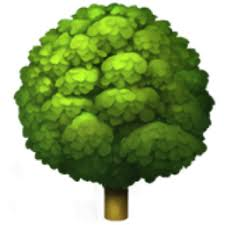
\includegraphics[height=1em]{tree1} \textcolor{blue}{is that they can supply fresh air
    for us.}

\item \textbf{So + \emph{a.} + be + S + that + ...}
  
  \textcolor{green}E. \textcolor{blue}{So precious is time that we can't afford to waste
it.}

\item \textbf{\emph{a.} + as + S + be, S + V.}

  \textcolor{green}E. \textcolor{blue}{Rich as our country is, the qualities of our living
    are by no means satisfactory.}

  \textcolor{red}{Note}. \textbf{by no means = in no way = on no account}

\item \textbf{The + \textasciitilde{er} + S + V, the + \textasciitilde{er} + S + V}
  
  \textbf{The + more + \emph{a.} + S + V, the + more + \emph{a.} + S + V}

  \textcolor{green}{E1}. \textcolor{blue}{The harder you work, the more progress you
    make.}

  \textcolor{green}{E2}. \textcolor{blue}{The more books we read, the more learned we
    become.}

\item \textbf{By + \emph{doing}, ...can...}

  \textcolor{green}E. \textcolor{blue}{By taking exercise, we can always stay healthy.}

\item \textbf{...enable + O + to + \emph{v.}}

  \textcolor{green}E. \textcolor{blue}{Listening to music enable us feel relaxed.}

\item \textbf{On no account can we + V}

  \textcolor{green}E. \textcolor{blue}{On no account can we ignore value of knowledge.}

\item \textbf{It is time + S + done}

  \textcolor{green}E. \textcolor{blue}{It is time the authorities concerned took proper
    steps to solve the traffic problems.}

\item \textbf{Those who...+ V}

  \textcolor{green}E. \textcolor{blue}{Those who violate traffic regulations should be punished.}

\item \textbf{There is no one but...}

  \textcolor{green}E. \textcolor{blue}{There is no one but longs to go to college.}

\item \textbf{be + forced/compelled/obliged + to \emph{v.}}

  \textcolor{green}E. \textcolor{blue}{Since the examination is around the corner, I am
    compelled to give up doing sports.}

\item \textbf{It is conceivable/obvious/apparent that... }

  \textcolor{green}E. \textcolor{blue}{It is conceivable that knowledge plays an
    important role in our life.}

\item \textbf{That is the reason why...}

  \textcolor{green}E. \textcolor{blue}{Summer is sultry. That is reason why I don't like it.}

\item \textbf{For the past + time, S + have done}

  \textcolor{green}E. \textcolor{blue}{For the past two years, I have been busy preparing
    for the examination.}

\item \textbf{Since + S + done, S + has done}

  \textcolor{green}E. \textcolor{blue}{Since he went to senior high school, he has worked
    very hard.}
  
\item \textbf{It pays to + \emph{v.}}

  \textcolor{green}E. \textcolor{blue}{It pays to help others.}

\item \textbf{be based on...}

  \textcolor{green}E. \textcolor{blue}{The progress of the society is based on harmony.}

\item \textbf{spare no effort + \emph{v.}}

  \textcolor{green}E. \textcolor{blue}{We should spare no effort to beautify our environment.}

\item \textbf{bring home to + somebody + something}

  \textcolor{green}E. \textcolor{blue}{We should bring home to people the value of working
  hard.}

\item \textbf{be closely related to...}

  \textcolor{green}E. \textcolor{blue}{Taking exercise is closely related to health.}

\item \textbf{get into the habit of \emph{doing} = make it a rule to \emph{v.}}

  \textcolor{green}E. \textcolor{blue}{We should get into the habit of keeping good hours.}

\item \textbf{Due to/Owing to/Thanks to + \emph{n./doing}}

  \textcolor{green}E. \textcolor{blue}{Thanks to his encouragement, I finally realized my dream.}

\item \textbf{What a/an + \emph{a.} + \emph{n.} + S + V}
  
    \textbf{How + \emph{a.} + a/an \emph{n.}  + S + V}

  \textcolor{green}{E1}. \textcolor{blue}{What an important thing it is to keep our
    promise.}

  \textcolor{green}{E2}. \textcolor{blue}{How important a thing it is to keep our promise.}

\item \textbf{...leave much to be desiblack}

  \textcolor{green}E. \textcolor{blue}{The condition of our traffic leaves much to be desiblack.}

\item \textbf{have a great influence on...}

  \textcolor{green}E. 
\includegraphics[height=1em]{smoking}\textcolor{blue}{ has a great
    influence on our health.}

\item \textbf{do good to.../do harm to...}

  \textcolor{green}{E1}. \textcolor{blue}{Reading does good to our mind.}

  \textcolor{green}{E2}. \textcolor{blue}{Overworking does harm to health.}

\item \textbf{pose a great threat to...}

  \textcolor{green}E. \textcolor{blue}{Pollution poses a great threat to our existence.}

\item \textbf{do one's utmost to + \emph{v.} = do one's best to \emph{v.}}

  \textcolor{green}E. \textcolor{blue}{We should do our utmost to achieve our
  }
\includegraphics[height=1.5em]{goal} \textcolor{blue}{in our life.}

  
  
\end{enumerate}

\begin{center}
  \section{INSPIRATIONAL QUOTES}
  \label{sec:inspirational-quotes}
\end{center}

\subsection{Education}
\label{sec:education}

\begin{itemize}
\item The roots of education are bitter, but the fruit is
  sweet.(\textcolor{cyan}{Aristotle})
  
\item Cultivation to the mind is as necessary as food for the
body. (\textcolor{yellow}{Cicero})
\end{itemize}


\subsection{Thinking}
\label{sec:thinking}

\begin{itemize}
\item Humanity needs practical men, but humanity also needs dreamers.
\item Science is organized knowledge. Wisdom is organized life.
\end{itemize}


\subsection{Life}
\label{sec:life}

\begin{itemize}
\item Life is a promise. Fulfill it.
\item Success is never final.(\textcolor{green}{Winston Churchill})
\end{itemize}

\subsection{Difficulty And Courage}
\label{sec:difficulty-courage}
\begin{itemize}
\item In the middle of difficulty lies opportunity.(\textcolor{red}{Albert Einstein})
\item Difficulties increase the nearer we get to the goal. (\textcolor{blue}{Goethe})
\end{itemize}

\subsection{Diligence}
\label{sec:diligence}

\begin{itemize}
\item The expectations of life depend upon diligence.(\textcolor{cyan}{Confucius})
\item Diligence is the mother of good luck.(\textcolor{green}{Thomas Fuller})
\end{itemize}

\subsection{Goals}
\label{sec:goals}

\begin{itemize}
\item If you want to live a happy life, tie it to the goal, not the people or the
  things.(\textcolor{red}{Albert Einstein})
\item To strive, to seek, to find, but not to yield.(\textcolor{blue}{Tennyson})
\end{itemize}

\subsection{Love}
\label{sec:love}

\begin{itemize}
\item The best and most beautiful things in the world cannot be seen or even touched. They
  must be felt with heart.(\textcolor{yellow}{Helen Keller})
\end{itemize}

\subsection{Teamwork}
\label{sec:teamwork}

\begin{itemize}
\item Divided we fall. United we stand.(\textcolor{cyan}{Lincoln})
\item As long as they think alike, a few people can move a mountain.
\end{itemize}


\begin{center}
  \section{VOCABULARY REPLACEMENT}
\end{center}

\hspace{-3cm}  \begin{tabular}{||c|>{\color{red}}c|c|>{\color{red}}c|c|>{\color{red}}c||}
                   \hline
                   Common Words& \textcolor{black}{Replacement}&Common
                                                                 Words&\textcolor{black}{Replacement}&Common Words&\textcolor{black}{Replacement} \\
                 \hline
                 
                 do, make & achieve & about & approximately & help & benefit \\
                 \hline
                 end, stop & conclude & prove, show & demonstrate & want & desire \\
                 \hline
                 show & exhibit & did not & failed to & for & for a period of \\
                 \hline
                 can & have the ability to & that is & i.e. & to & in order to \\
                 \hline
                 soon & in the near future & find & locate & let me know & notify \\
                 \hline
                 many & numerous & get & obtain & tell & advise \\
                 \hline
                 try & attempt & start,begin & commence & give & contribute \\
                 \hline
                 leave & depart & stop & discontinue & skill, ability & expertise \\
                 \hline
                 complete, finish & finalize & these & the following & here & herein \\
                 \hline
                 besides & in addition & about & in  regard to & last, finally & last but
                                                                                 not least
               \\
                 \hline
                 most & the majority & by & not later than & see & observe \\
                 \hline
                 do & perform & people & personnel & ready & prepared \\
                 \hline
                 chance & probability & buy & purchase & about & relative to \\
                 \hline
                 ask & request & like & similar to & send & submit \\
                 \hline
                 end,stop & terminate & send & transmit & about & with reference to \\
                 \hline
                 own & possess & before & prior to & if & provided that \\
                 \hline
                 about & regarding & rest & reminder & second & secondly \\
                 \hline
                 say & state & enough & sufficient & so & therefore \\
                 \hline
                 use & utilize & I,me & the writer & important & crucial \\
                 \hline
                 common & universal & abundant & ample & difficult & arduous \\
                 \hline
                 show & demonstrate & always & invariably & boring & tedious \\
                 \hline
                 nowadays & currently & only & unique & stop & cease \\
                 \hline
                 based on & derived from & change & convert & ability & capacity \\
                 \hline
                 despite & notwithstanding & possible & feasible & so & consequently \\
                 \hline
                 
                   
  \end{tabular}



\begin{center}
\hspace{3cm}  \section{THE END}
\label{sec:end}

\end{center}

\hspace{3.5cm} \Shapepar{\circleshape} Thank you the authors, \textcolor{red}{Qiyuan Pu},
\textcolor{green}{Zhicheng Yin}, \textcolor{blue}{Yuanmeng Liu}, all patients, energy and
focus of yours make this created, especially all of you during the preparing for exam.
The best wishes for you. 
\includegraphics[height=1em]{thanks}

\begin{center}
  Of course, and you \LaTeX{}, you are really nice typesetting tool yet looking like a bit
  ugly,  just a bit.
\includegraphics[height=1.3em]{grimace}

  And 
\includegraphics[height=2em]{google}, you always stays with me, my forever friend,
  thanks for your help every time when I puzzled.
\end{center}


\end{document}
 



%%% Local Variables:
%%% mode: latex
%%% TeX-master: t
%%% End:
